\begin{center}
    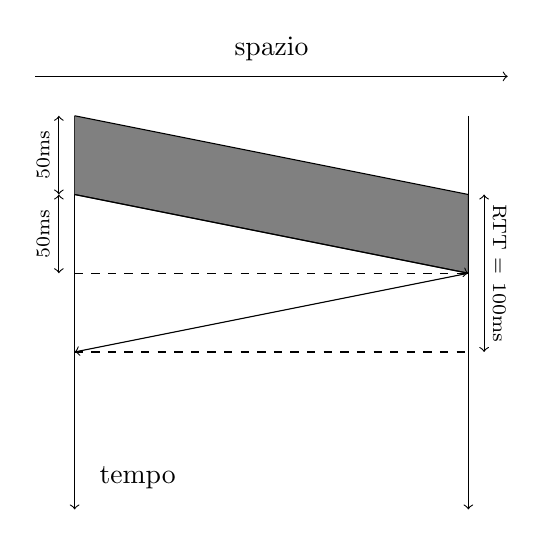
\begin{tikzpicture}
        % Vettore e testo per lo spazio
        \node[align=center] at (2.5,0.85) {spazio};
        \draw[->] (-0.5,0.5) -- (5.5,0.5);

        % Vettori e testo per il tempo
        \node at (0.8,-4.6) {tempo};
        \draw[->] (0,0) -- (0,-5);
        \draw[->] (5,0) -- (5,-5);

        % Scambio di messaggi
        \draw[fill=gray] (0,0) -- (5,-1) -- (5,-2) -- (0,-1);
        \draw[->] (0,-1) -- (5,-2);
        \draw[->] (5,-2) -- (0,-3);

        % Tratteggio di riferimento
        \draw[dashed] (0,-2) -- (5,-2);
        \draw[dashed] (0,-3) -- (5,-3);

        % Misurazioni
        \draw[<->] (-0.2, 0) -- (-0.2, -1);
        \node[rotate=90] at (-0.4,-0.5) {\scriptsize 50ms};
        \draw[<->] (-0.2, -1) -- (-0.2, -2);
        \node[rotate=90] at (-0.4,-1.5) {\scriptsize 50ms};
        \draw[<->] (5.2, -1) -- (5.2, -3);
        \node[rotate=270] at (5.4,-2) {\scriptsize RTT = 100ms};
    \end{tikzpicture}
\end{center}